\begin {tikzpicture}
	\node[draw,align=center] (in) at(0,0) {Eingabebild\\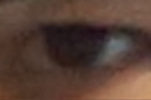
\includegraphics[width=0.18\linewidth]{img_Versuch_Auge/Auge_in}};
	\node[draw,align=center] (El) at(6,0)  {Ellipse\\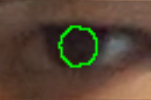
\includegraphics[width=0.18\linewidth]{img_Versuch_Auge/Auge_EL}};
	\node[draw,align=center] (OF) at(6,-4) {Landmark\\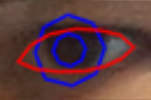
\includegraphics[width=0.18\linewidth]{img_Versuch_Auge/Auge_OF}};
	\node[draw,align=center] (ER) at(12,0)  {Ergebnis\\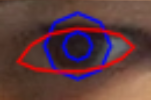
\includegraphics[width=0.18\linewidth]{img_Versuch_Auge/Auge_ER}};
		
	\draw[->] (in)to node[above]{ElSe}(El);
	\draw[->] (in)to node[left]{OpenFace}(OF);
	
	\draw[->] (El)to node[above]{Iris \& Pupille}(ER);
	\draw[->] (OF)to node[right]{Augenlider}(ER);	
\end{tikzpicture}